\documentclass[hidelinks]{report}

\usepackage[utf8]{inputenc} % Character encoding
\usepackage[english]{babel} % Language

\usepackage[table,xcdraw]{xcolor} % Table colors
\usepackage{tabularx} % Dynamic table width
\usepackage{tcolorbox} % Gray boxes
\usepackage{hyperref} % URL environment
\usepackage{todonotes} % Notes
\usepackage{natbib} % Bibliography
\usepackage{fancyhdr} % Header and footer
\usepackage{multirow} % Multirow
\usepackage{geometry} % Page layout
\usepackage{color} % Text colors
\usepackage{float} % Show tables within their section
\usepackage{listings} % Code
\usepackage{pdflscape} % Horizontal orientation (landscape)

% Command for inline code
\newcommand{\code}[1]{\lstinline[language=json,columns=fixed,breakatwhitespace]{#1}}

% Commands for requirements priorities
\newcommand{\priohigh}{1 - high}
\newcommand{\prioavg}{2 - average}
\newcommand{\priolow}{3 - low}
\newcommand{\prioopt}{4 - optional}

% JSON display
\colorlet{punct}{red!60!black}
\definecolor{background}{HTML}{EEEEEE}
\definecolor{delim}{RGB}{20,105,176}
\colorlet{numb}{magenta!60!black}

\lstdefinelanguage{json}{
    basicstyle=\normalfont\ttfamily,
    numbers=left,
    numberstyle=\scriptsize,
    stepnumber=1,
    numbersep=8pt,
    showstringspaces=false,
    breaklines=true,
    frame=lines,
    backgroundcolor=\color{background},
    literate=
     *{0}{{{\color{numb}0}}}{1}
      {1}{{{\color{numb}1}}}{1}
      {2}{{{\color{numb}2}}}{1}
      {3}{{{\color{numb}3}}}{1}
      {4}{{{\color{numb}4}}}{1}
      {5}{{{\color{numb}5}}}{1}
      {6}{{{\color{numb}6}}}{1}
      {7}{{{\color{numb}7}}}{1}
      {8}{{{\color{numb}8}}}{1}
      {9}{{{\color{numb}9}}}{1}
      {:}{{{\color{punct}{:}}}}{1}
      {,}{{{\color{punct}{,}}}}{1}
      {\{}{{{\color{delim}{\{}}}}{1}
      {\}}{{{\color{delim}{\}}}}}{1}
      {[}{{{\color{delim}{[}}}}{1}
      {]}{{{\color{delim}{]}}}}{1},
}

% Cucumber.
\lstdefinelanguage{Gherkin}{
  keywords={When, Then, Given, And},
  ndkeywords={Feature, Scenario},
  sensitive=true,
  comment=[l]{!--},
  morestring=[b]"
}

% Configure page layout
% Page layout
\geometry{
	bottom=3.5cm,
	headheight=180pt
}

% Nummerierung der ersten Seiten verhindern
\pagenumbering{gobble}

% Bibstyle
\bibliographystyle{plain}

% Header / Footer
\fancypagestyle{plain}{
	\fancyhf{}% Clear header/footer
	\fancyhead[R]{
\includegraphics[width=4cm]{img/aa-logo}} % Rechter header
	\fancyhead[L]{\leftmark} % Linker header
	\fancyfoot[R]{\thepage} % Rechter footer
}
\pagestyle{plain}

\renewcommand{\headrulewidth}{0.5pt} % Unnötige Informationen der Kapitelangabe
\renewcommand{\footrulewidth}{0.2pt} % entfernen
\renewcommand{\chaptermark}[1]{\markboth{{#1}}{}}

% Zahlen für Fußnoten
\renewcommand{\thefootnote}{\arabic{footnote}}
\renewcommand{\thempfootnote}{\arabic{mpfootnote}}


% Title page
% Document name
\newcommand{\documentname}{Technical documentation}
\newcommand{\documentVersion}{2.0}

% Project name
\newcommand{\projectNameShort}{VRGP}
\newcommand{\projectNameLong}{VRGP implementation for the Åboat}
\newcommand{\projectName}{{\projectNameLong} (\projectNameShort)}

% Course name
\newcommand{\course}{Project course}
\newcommand{\semester}{2021 - 2022}

% Gruppenmitgieder.
\makeatletter
\newcommand{\memberOne}   {Md Hredoy Mesha & \href{mailto:meshahredoy@gmail.com}{meshahredoy@gmail.com}}
\newcommand{\memberTwo}   {Gabriela Corbalan Gomez & \href{mailto:gabri.corba@gmail.com}{gabri.corba@gmail.com}}
\newcommand{\memberThree} {Daniel Gonzálves Alfert & \href{mailto:danielgalfert@gmail.com}{danielgalfert@gmail.com}}
\newcommand{\memberFour}  {Alexandru Gherghescu & \href{mailto:alexandru.gherghescu@abo.fi}{alexandru.gherghescu@abo.fi}}
\newcommand{\memberFive}  {Joan Dolz Mensua & \href{mailto:joan.dolzmensua@abo.fi}{joan.dolzmensua@abo.fi}}
\newcommand{\memberSix}   {Elijah Rose & \href{mailto:elijah.rose@abo.fi}{elijah.rose@abo.fi}}
\newcommand{\memberSeven} {Yannick Zapfe & \href{mailto:yannick.zapfe@abo.fi}{yannick.zapfe@abo.fi}}
\makeatother

\title{
	\vspace*{-3cm}
	\projectName\\
	\documentname\\
	Version \documentVersion\\
	-\\
	\color{gray}
	\course\ \semester\\
	\vspace*{5mm}
	
\includegraphics[width=0.5\textwidth]{img/vrgp-logo}
}

\author{
	\begin{tabular}{r l@{\hspace{7\tabcolsep}} r}
		\memberOne   \\
		\memberTwo   \\
		\memberThree \\
		\memberFour  \\
		\memberFive  \\
		\memberSix   \\
		\memberSeven
	\end{tabular}
}

\date{\today}


% Document

\begin{document}
	\maketitle

	\chapter*{Revision history}

	\begin{table}[H]
		\centering
		\begin{tabularx}{\textwidth}{ l c X }
			\rowcolor[HTML]{C0C0C0}
			\textbf{Date} & \textbf{Version} & \textbf{Description} \\
			20.10.2021 & 1.0 & Initial version \\
			\rowcolor[HTML]{E7E7E7}
			11.11.2021 & 2.0 & Initial design \\
			17.11.2021 & 2.1 & Translation to LaTeX \\
			\rowcolor[HTML]{E7E7E7}
			03.02.2022 & 3.0 & Components update \\
		\end{tabularx}
	\end{table}

	\tableofcontents

	\chapter{Product Requirements}\label{chp:requirements}
	\pagenumbering{arabic} % Start page numbering.
	\thispagestyle{fancy}
	The purpose of the VRGP is to provide a standardized way of communication for vessels and Maritime Operating Centres (MOC) on the shore. Most importantly, VRGP includes streaming live data from the vessel to the shore and, based on this data, sending guidance messages from the shore to the vessel. This system, a VRGP implementation for the Åboat and, therefore, a maritime system, serves as a proof of concept of the protocol specification and standardizes the external communication of the Åboat.
\\\\
The VRGP implementation will provide the Åboat with the functionality described in the protocol specification, an interface for communication with a MOC. This includes initiating and creating a connection with a MOC, streaming on-board information upon request, terminating a connection, sending notification about abnormal situations on board and receiving guidance from the MOC. The VRGP implementation will be integrated into the existing Åboat architecture and connect with its user interface.
\\\\
The implementation can also be used as a starting point for other implementations. Parts of it will be reusable and the core implementation may even be an independent component to be used by other vessels than the Åboat.

\section{Functional Requirements}\label{sec:func-requirements}

\begin{figure}[ht]
	\centering
	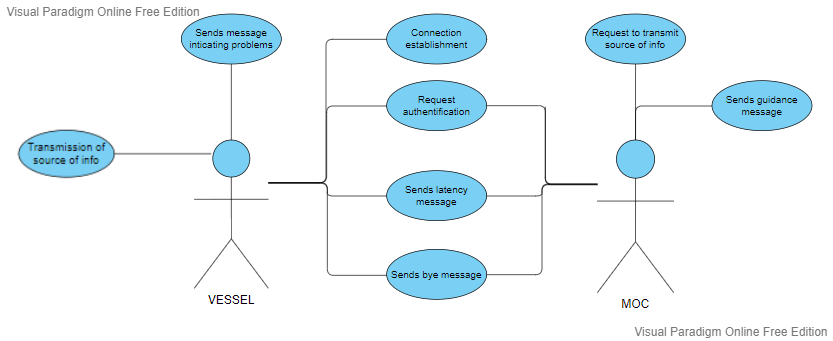
\includegraphics[width=\linewidth]{uml/use-case-diagram}
	\caption{Use case diagram}
	\label{fig:use-case-diagram}
\end{figure}

\subsection{Initiate Connection}

\subsection{Information Streams}

\subsection{Terminate Connection}

\subsection{Authentication}

\subsection{Messages about problems on board}

\subsection{Latency}

\subsection{Clock synchronisation}

\subsection{Guidance}

\section{User Interface Requirements}\label{sec:ui-requirements}

\section{Non-functional Requirements}\label{sec:non-func-requirements}

\subsection{Deliverable}

\subsection{Security}

\subsection{Availability}


	\chapter{System Architecture and Design}\label{chp:design}
	\thispagestyle{fancy}
	\section{Architecture}\label{sec:architecture}

The Åboat already has an architecture of its own. The system is already functional (though it has its own communication protocol). What we aim to do is build on top of this architecture.
\\\\
Currently, the Åboat has an architecture that consists of microservices. Each of these microservices runs a different “functionality” of the boat. There are microservices for sensors, control, storage, and communication. The current picture of the Åboat architecture can be seen in the image below.

\begin{figure}[ht]
	\centering
	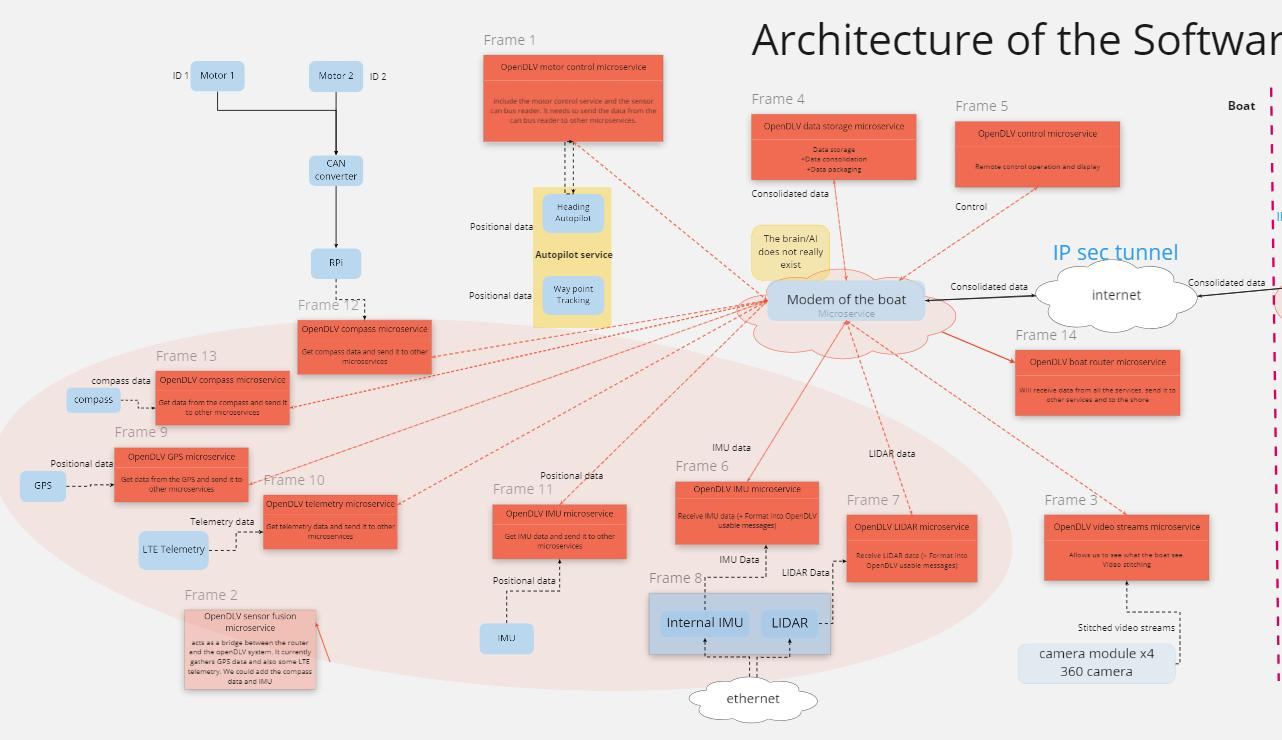
\includegraphics[width=\linewidth]{images/aboat-architecture}
	\caption{Åboat architecture}
	\label{fig:aboat-architecture}
\end{figure}

The purpose of the VRGP implementation is to create an independent system implementing the VRGP specification, which will interface with the existing architecture of the Åboat. The interfacing will be achieved through a microservice (called an \textbf{adapter}), which has the sole purpose of translating the calls between the Åboat and the VRGP service. This will make the VRGP service completely independent of the vessel that uses it, thus achieving a good level of decoupling.
\\\\
Using the VRGP service with other boats would then be easy, as the only component that would have to be rewritten would be the \textbf{adapter}, which, as mentioned above, is only a small layer that interfaces between the vessel and VRGP service.
\\\\
On the shore-side, there is the MOC service, which consists of a backend and frontend. The backend is responsible for the communication with the vessel-side (more specifically, the VRGP service), while the frontend is responsible for displaying the information to (most likely) human operators.
\\\\
An image of the current architecture of the VRGP implementation can be seen below.

\begin{figure}[ht]
	\centering
	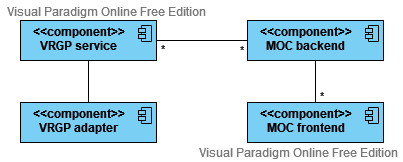
\includegraphics[width=\linewidth]{images/vrgp-architecture}
	\caption{VRGP architecture}
	\label{fig:vrgp-architecture}
\end{figure}

More details about the components are presented in the implementation section below (section \ref{sec:technologies}).

\section{Design}\label{sec:design}

In the following sections, we describe our current design using several UML diagrams. UML is used for most parts of the design for now, as it provides a well-known, easy to understand and somewhat unambiguous description of the design. Some of the diagrams present the high-level views of the system, while others are more in-depth.

\subsection{Static Design}

\subsubsection{Deployment Diagram}

The deployment diagram provides an overview of the different deliverables for this software project and in which environments they can be used. The most important artifact to be delivered is the VRGP service (which is the actual VRGP implementation), while the other deliverables (the OpenDLV adapter, the MOC backend and frontend) are mostly built around the service and aim to show that it works. The deployment diagram is shown in figure \ref{fig:deployment-diagram}.

\begin{figure}[ht]
	\centering
	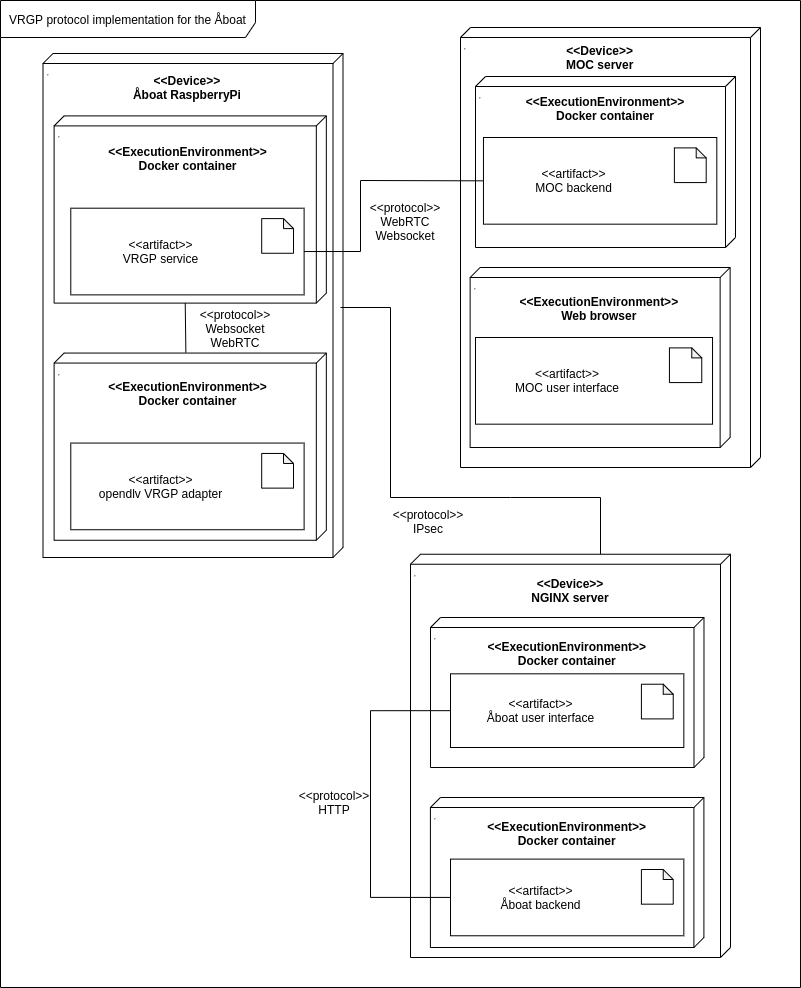
\includegraphics[width=\linewidth]{diagrams/deployment-diagram}
	\caption{Deployment diagram}
	\label{fig:deployment-diagram}
\end{figure}

\subsubsection{Component Diagrams}

The high-level components have been briefly described in the introduction above.
\\\\
The most important part of the communication happens between the vessel-side and the shore-side, i.e. between the VRGP service and the MOC. A diagram illustrating this connection can be seen in figure \ref{fig:vrgp-moc-component-diagram}.
\\\\
As can be seen, the component diagram mostly follows the requirements outlined above (\ref{sec:func-requirements}).
\\\\
Another important part of the communication happens between the VRGP service and the adapter microservice. The communication can be seen in figure \ref{fig:adapter-vrgp-component-diagram}.
\\\\
The left side depicts the OpenDLV microservice running the adapter, which will have further communications with the other Åboat microservices.

\begin{figure}[h!]
	\centering
	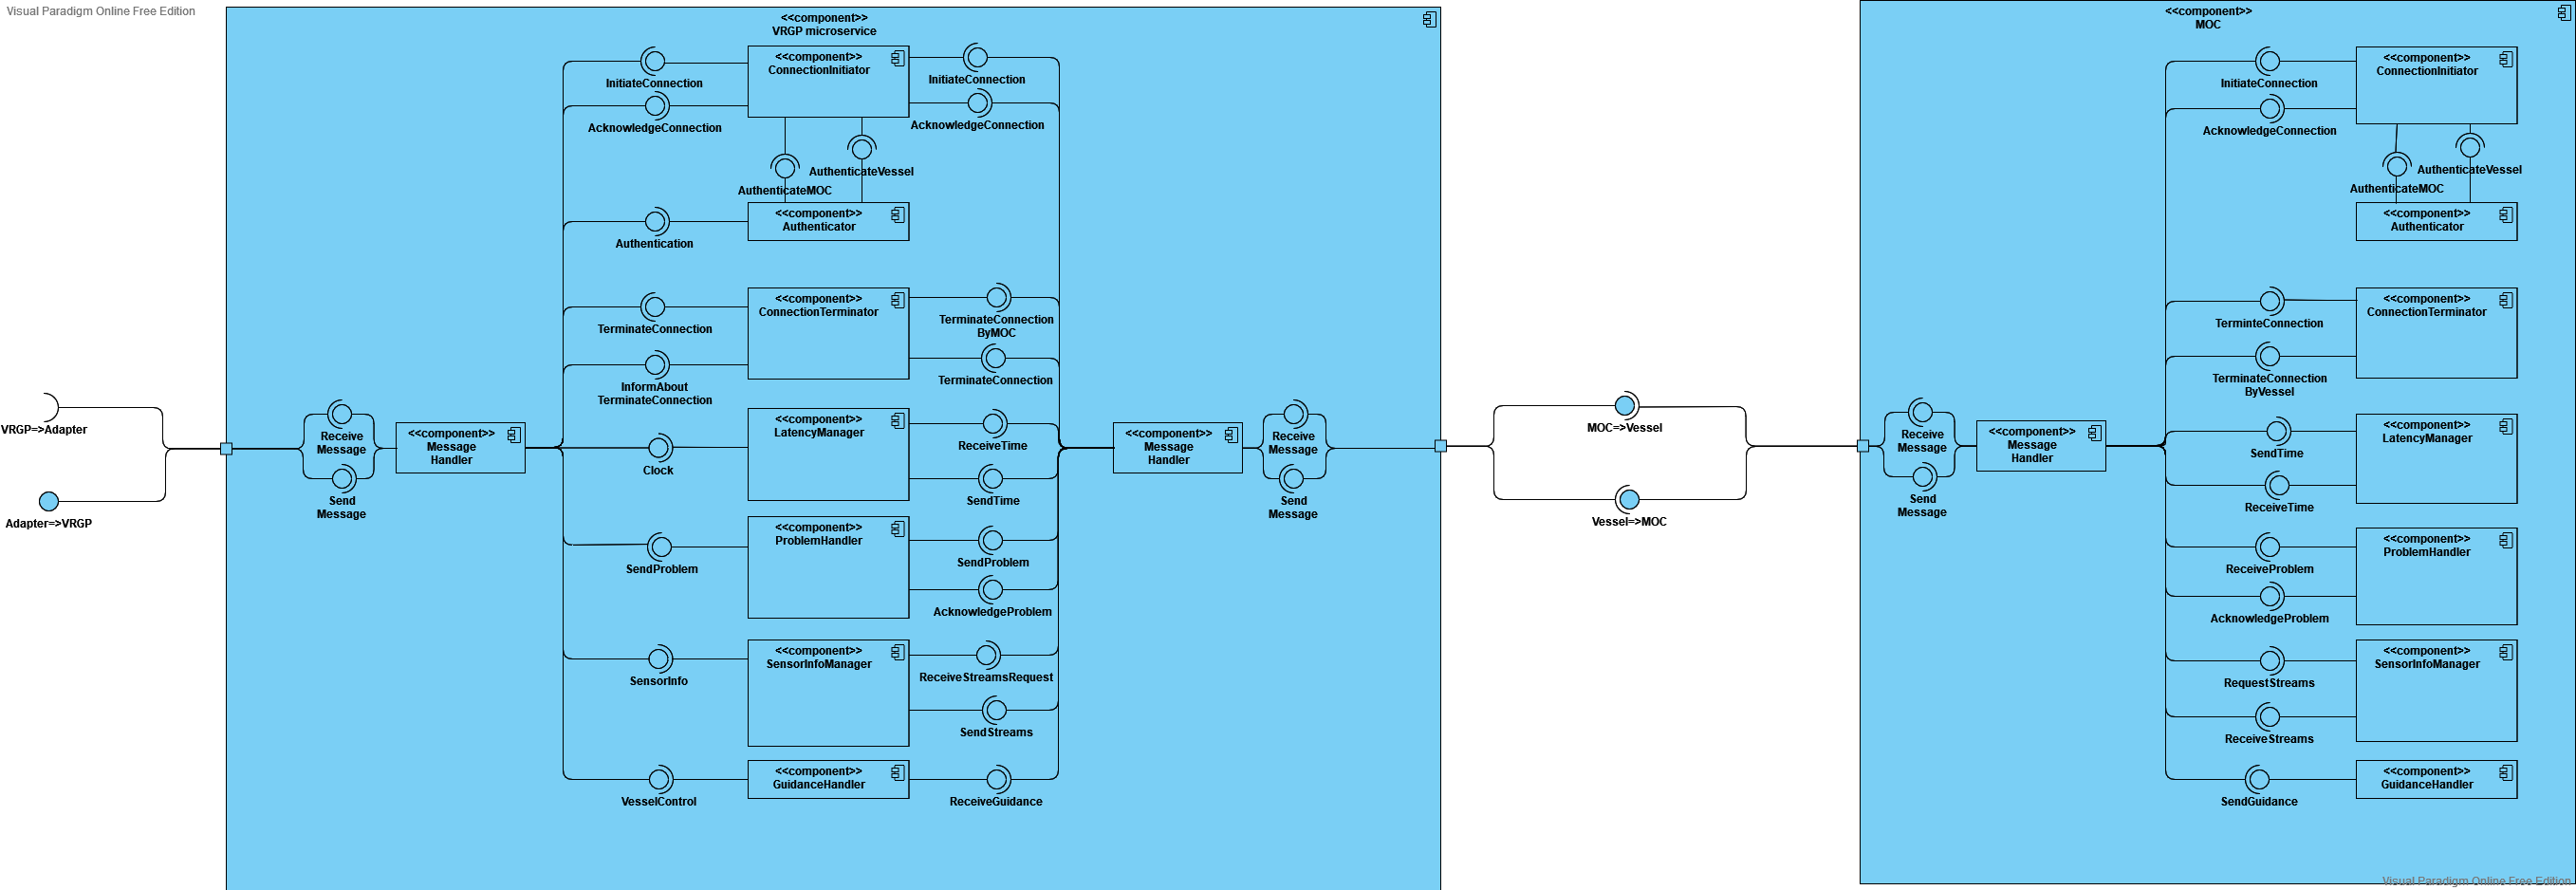
\includegraphics[width=\linewidth]{diagrams/ComponentDiagram_GenericVrgpMicroservice_HandlerView}
	\caption{VRGP service - MOC component diagram}
	\label{fig:vrgp-moc-component-diagram}
\end{figure}

\begin{figure}[h!]
	\centering
	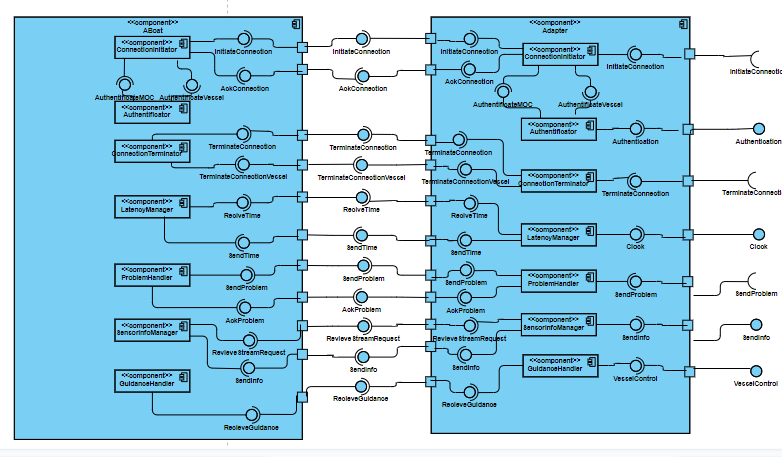
\includegraphics[width=\linewidth]{diagrams/components_adapter}
	\caption{Åboat adapter - VRGP service component diagram}
	\label{fig:adapter-vrgp-component-diagram}
\end{figure}

\subsection{Dynamic Design}\label{sec:dynamic-design}

\subsubsection{Activity Diagram}

This high-level activity diagram (figure \ref{fig:activity-diagram}) provides an overview of the general communication flow in the VRGP protocol, including the connection establishment and authentication, the messages that can be sent continuously while the connection is up and the termination of the connection. In further steps, this diagram will either be refined to account for more details of the protocol or split into multiple activity diagrams to depict the different processes in more detail.

\begin{figure}[ht]
	\centering
	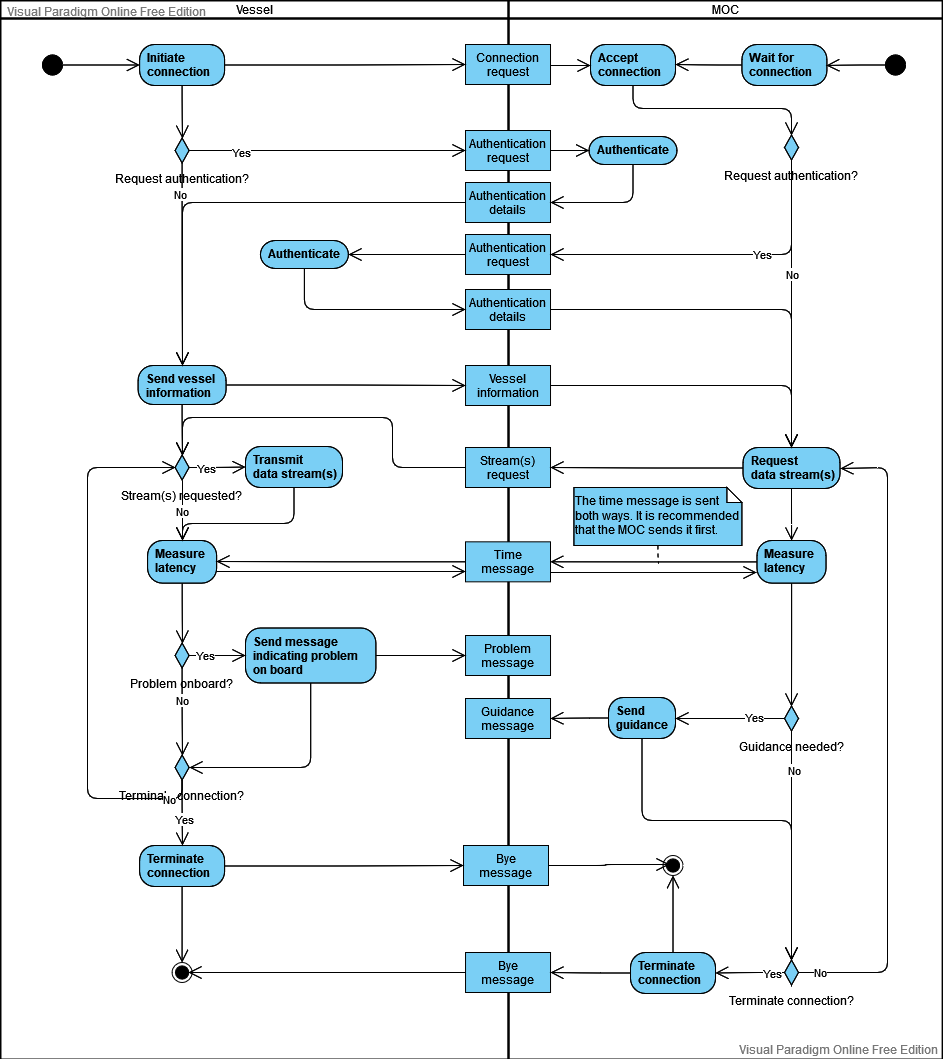
\includegraphics[width=\linewidth]{diagrams/activity-diagram}
	\caption{Activity diagram}
	\label{fig:activity-diagram}
\end{figure}

\subsubsection{Sequence Diagram}

In another design refinement step, sequence diagrams for different processes and sub-processes will be developed to clearly define the communication flow and how it will be implemented in the software using the components and classes we defined in \ref{sec:dynamic-design}.


	\chapter{Implementation}\label{chp:implementation}
	\thispagestyle{fancy}
	\section{Technologies}\label{sec:technologies}

The languages and technologies used are mainly those imposed by the already existing Åboat infrastructure. For the vessel side (i.e. the actual system implementation that will run as a microservice along with the boat’s existing software), the technologies used are:

\begin{itemize}
	\item C++ and OpenDLV (microservices solution)
	\item WebSockets and WebRTC (communication protocols for data over the internet)
	\item Docker (container solution)
	\item Raspberry Pi, LIDAR, GPS, radar, compass, and other existing hardware equipment
\end{itemize}

\noindent
Additionally, there is going to be a web interface as a way to test the VRGP connection to the vessel. Åboat currently has a web interface capable of streaming some data from the vessel to the shore. That interface will be extended by this project. The technologies that will be used in this regard are:

\begin{itemize}
	\item Web technologies (HTML, CSS, JavaScript)
\end{itemize}


	\chapter{References}\label{chp:references}
	\thispagestyle{fancy}
	The official VRGP specification can be found on \href{https://github.com/aboamare/vrgp-specifications/blob/master/Protocol\%20specification.md}{GitHub}.
\\\\
The OpenDLV website can be found \href{https://opendlv.org}{here}. 


	\chapter{Terminology}\label{chp:terminology}
	\thispagestyle{fancy}
	\begin{tabular}{rl}
	VRGP: & Vessel Remote Guidance Protocol \\
	MOC: & Maritime Operating Center \\
	MCP: & Maritime Connectivity Platform
\end{tabular}

\end{document}
